\chapter{Đối ngẫu T, D-brane và lý thuyết chuẩn}

\lectureoverview{Đối ngẫu T khởi đầu như một sự tương đương chính xác giữa các dây kín trên các đường tròn có bán kính (R) và \(\alpha'/R\). Xung lượng và số quấn hoán đổi vai trò cho nhau, cũng như các đạo hàm worldsheet \(\partial_\tau Y\) và \(\partial_\sigma Y\), và các vectơ không-thời gian suy ra từ \(G_{\mu 5}\) và \(B_{\mu 5}\). Khi áp dụng cùng phép biến đổi ấy cho một dây mở, một điều kiện biên Neumann ở đầu mút trở thành một điều kiện Dirichlet. Khi đó đầu mút phải nằm trên một D-brane động lực học. Các dây mở bị giam trên một brane sinh ra một lý thuyết chuẩn abel ở năng lượng thấp; các dây nối một chồng brane mang hai nhãn đầu mút và sinh ra một lý thuyết chuẩn không abel. Một D-string kết thúc trên một D3-brane cung cấp đơn cực từ tương ứng.}

\section{Vì sao quay lại với đối ngẫu T?}

Chúng ta đã gặp đối ngẫu T rồi, nhưng có lý do để quay lại với nó. Đó là một trong những manh mối cho thấy lý thuyết dây chứa nhiều hơn rất nhiều so với các dây nhiễu loạn. Một khi các hệ quả của nó đối với dây mở được hiểu rõ, nó đã dẫn tới D-brane; đến lượt mình, D-brane trở thành một cách xây dựng và nghiên cứu các lý thuyết trường lượng tử. Vì vậy, mục tiêu của bài giảng này không chỉ đơn thuần là lặp lại khẩu hiệu rằng một đường tròn nhỏ tương đương với một đường tròn lớn. Chúng ta sẽ dựng lại lập luận đủ cẩn thận để thấy khẩu hiệu ấy buộc lý thuyết phải đưa vào những đối tượng vật lý mới như thế nào.

Bối cảnh đơn giản nhất là compact hóa xuyến. Một xuyến một chiều là một đường tròn. Một xuyến hai chiều có thể được biểu diễn bằng một hình bình hành với các cạnh đối diện được đồng nhất, và một xuyến ba chiều bằng một hình hộp xiên với các mặt đối diện được đồng nhất. Cùng phép dựng đó tiếp tục trong số chiều cao hơn. Ta sẽ chỉ giữ lại một tọa độ không gian compact, gọi là \(Y\), và một tọa độ không compact đại diện, gọi là \(X\). Thời gian có mặt nhưng không được vẽ trong các hình trên bảng.

Chọn quy ước chuẩn
\begin{equation}
  Y\sim Y+2\pi R,
  \label{eq:l10-circle-identification}
\end{equation}
để \(R\) là bán kính và \(2\pi R\) là chu vi. Trong bài giảng, kích thước compact thường được gọi đơn giản là \(r\) và lược bỏ các thừa số \(2\pi\) và \(\alpha'\). Ta sẽ giữ lại các thừa số quy ước trong các phép suy diễn và hiển thị các đơn vị của bài giảng khi chúng hữu ích.

Trong nửa đầu của phần thảo luận, các dây là kín và có định hướng. Định hướng là một mũi tên nội tại vẽ dọc theo dây. Đảo ngược mọi mũi tên ở khắp nơi sẽ không làm thay đổi thí nghiệm nào; điều quan trọng là định hướng tương đối của hai dây. Trong quá trình tách và nhập, các mũi tên phải nối với nhau một cách liên tục. Đây là gợi ý đầu tiên rằng sẽ xuất hiện một đại lượng bảo toàn có dấu.

\begin{figure}[H]
  \centering
  \includegraphics[width=0.72\textwidth]{lecture_10_figure_01.png}
  \caption{Hai dây kín với định hướng tương đối của chúng được đánh dấu trên bảng. Định hướng phải liên tục qua các quá trình tách và nhập.}
  \lectureframe{00:05:40}
  \label{fig:l10-oriented-closed-strings}
\end{figure}

\begin{classroomqa}
\audiencequestion{Nếu tọa độ worldsheet chạy từ \(\sigma=0\) đến \(2\pi\), thì dây đã đi trọn một vòng quanh phương compact chưa? \lecturetimestamp{00:08:42}}
\lecturerresponse{Chưa. Tọa độ \(\sigma\) gán nhãn các điểm dọc theo dây; nó không gán nhãn các vị trí trong không gian compact. Mọi dây kín đều có một tham số tuần hoàn \(\sigma\), dù nó có quấn hay không quấn. Phép ví von với dây chun rất hữu ích: ta có thể đánh số các phân tử quanh một vòng dây chun ngay cả khi vòng đó không quấn quanh vật gì. Sự quấn là một tính chất của ánh xạ \(Y(\tau,\sigma)\), chứ không phải chỉ riêng của tham số \(\sigma\).}
\end{classroomqa}

\begin{classroomqa}
\audiencequestion{Kích thước compact cũng có phải là như nhau tại mọi giá trị của tọa độ lớn \(X\) không? \lecturetimestamp{00:10:00}}
\lecturerresponse{Không phải trong một compact hóa động lực học tổng quát. Ta bắt đầu với một đường tròn cố định vì đó là nền đơn giản nhất. Về sau, thành phần \(G_{55}\) sẽ trở thành một trường vô hướng mà giá trị của nó đo kích thước cục bộ của chiều thứ năm, vì thế kích thước đó có thể biến thiên trên không-thời gian thông thường.}
\end{classroomqa}

\section{Số quấn được bảo toàn ngay cả khi các dây tái nối}

Một dây không quấn có thể chuyển động qua phương compact mà không quấn quanh nó. Một dây có quấn thì khác: khi \(\sigma\) đi một vòng quanh dây kín, phép nhúng \(Y(\tau,\sigma)\) tiến qua một hay nhiều chu kỳ của đường tròn compact. Vì dây có định hướng nên sự tiến này có dấu. Một dây có thể quấn theo chiều dương hoặc theo chiều âm.

Định luật bảo toàn được thấy rõ nhất trong các hình ghép nối. Lấy một dây có số quấn \(+1\) và một dây khác có số quấn \(-1\). Các đoạn tương hợp của chúng có thể tái nối. Cấu hình thu được có tổng số quấn bằng không và có thể bị biến dạng thành một dây không quấn. Hình vẽ trên bảng lần theo chính xác sự tái nối với định hướng đối nhau này.

\begin{figure}[H]
  \centering
  \includegraphics[width=0.72\textwidth]{lecture_10_figure_02.png}
  \medskip

  \begin{tikzpicture}[x=1cm,y=1cm,>=Latex]
    \draw[thick] (-4.0,0.3) circle (0.65);
    \draw[->,thick] (-4.55,0.58) arc (150:-145:0.65);
    \node at (-4.0,-0.65) {$w=+1$};
    \draw[thick] (-2.0,0.3) circle (0.65);
    \draw[<-,thick] (-2.55,0.58) arc (150:-145:0.65);
    \node at (-2.0,-0.65) {$w=-1$};
    \node at (-3.0,0.3) {$+$};
    \draw[->,thick] (-1.0,0.3) -- (0.3,0.3);
    \draw[thick] (1.4,0.3) ellipse (0.95 and 0.55);
    \node at (1.4,-0.65) {$w_{\rm total}=0$};
  \end{tikzpicture}
  \caption{Hai số quấn đối nhau tái nối thành một cấu hình có tổng số quấn bằng không. Hình dưới là bản dựng lại gọn gàng của thao tác trên bảng, không phải một quá trình động lực học thứ hai.}
  \lectureframe{00:13:20}
  \label{fig:l10-opposite-winding}
\end{figure}

Bây giờ lặp lại thí nghiệm với hai dây có cùng định hướng. Chúng có thể nhập lại, nhưng không thể tháo quấn. Kết quả mang số quấn gấp đôi mỗi dây ban đầu. Số dây liên thông đã thay đổi; tổng số quấn thì không.

\begin{figure}[H]
  \centering
  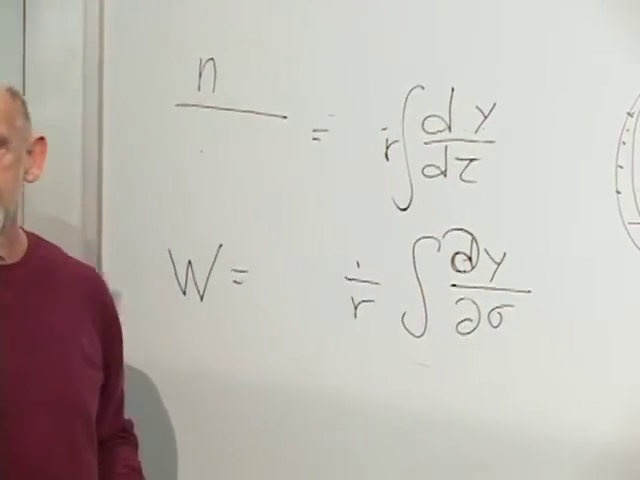
\includegraphics[width=0.72\textwidth]{lecture_10_figure_03.png}
  \medskip

  \begin{tikzpicture}[x=1cm,y=1cm,>=Latex]
    \draw[thick] (-4.0,0.3) circle (0.65);
    \draw[->,thick] (-4.55,0.58) arc (150:-145:0.65);
    \node at (-4.0,-0.65) {$w=+1$};
    \draw[thick] (-2.0,0.3) circle (0.65);
    \draw[->,thick] (-2.55,0.58) arc (150:-145:0.65);
    \node at (-2.0,-0.65) {$w=+1$};
    \node at (-3.0,0.3) {$+$};
    \draw[->,thick] (-1.0,0.3) -- (0.3,0.3);
    \draw[thick] (1.45,0.3) circle (0.78);
    \draw[thick] (1.45,0.3) circle (0.52);
    \draw[->,thick] (0.81,0.74) arc (145:-145:0.78);
    \node at (1.45,-0.78) {$w=+2$};
  \end{tikzpicture}
  \caption{Các số quấn cùng dấu có thể tái nối thành một dây quấn hai lần. Tính liên thông thay đổi trong khi tổng số quấn vẫn là hai.}
  \lectureframe{00:16:40}
  \label{fig:l10-same-winding}
\end{figure}

Sự phân biệt này còn đúng trong mọi quá trình được phép. Tổng số quấn một trăm có thể được mang bởi một dây quấn một trăm vòng, hai dây mỗi dây quấn năm mươi vòng, hoặc một trăm dây mỗi dây quấn một vòng. Các dây có thể tách và nhập giữa các mô tả này, nhưng tổng có dấu vẫn là một trăm. Ta ký hiệu nó bởi \(w\in\mathbb Z\).

\section{Các mode xung lượng và các mode quấn}

Bản thân sự bảo toàn vẫn chưa phải là đối ngẫu. Tiếp theo ta so sánh các năng lượng. Một trạng thái chuyển động quanh đường tròn compact có xung lượng lượng tử hóa
\begin{equation}
  p_Y=\frac{n}{R},
  \qquad n\in\mathbb Z.
  \label{eq:l10-compact-momentum}
\end{equation}
Đối với một trạng thái mà các đóng góp khác vào khối lượng có thể bỏ qua, chuyển động theo phương compact đóng góp \(E_{\rm mom}=|n|/R\). Các giá trị dương và âm của \(n\) biểu thị hai chiều chuyển động ngược nhau, còn năng lượng thì dương.

\begin{figure}[H]
  \centering
  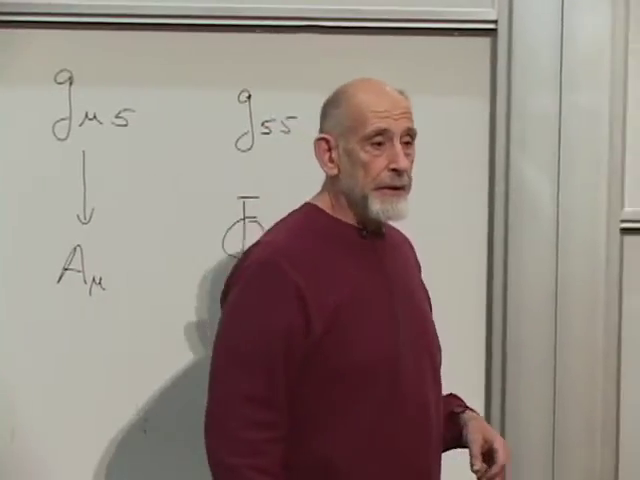
\includegraphics[width=0.72\textwidth]{lecture_10_figure_04.png}
  \caption{Số lượng tử xung lượng compact trên bảng. Bài giảng viết xung lượng một cách sơ đồ như một tích phân của vận tốc theo phương compact.}
  \lectureframe{00:21:30}
  \label{fig:l10-compact-momentum-board}
\end{figure}

Một dây quấn \(|w|\) lần có độ dài \(2\pi |w|R\). Với lực căng của dây cơ bản
\begin{equation}
  T_{\rm F}=\frac{1}{2\pi\alpha'},
\end{equation}
năng lượng quấn của nó là
\begin{equation}
  E_{\rm wind}=T_{\rm F}(2\pi |w|R)
  =\frac{|w|R}{\alpha'}.
  \label{eq:l10-winding-energy}
\end{equation}
Trong đơn vị của bài giảng \(\alpha'=1\), điều này đơn giản là \(E_{\rm wind}=|w|R\).

Hai tháp mức này ứng xử ngược nhau khi bán kính thay đổi. Với \(R\gg
\sqrt{\alpha'}\), các mức xung lượng nằm sít nhau còn các mức quấn thì thưa. Với \(R\ll\sqrt{\alpha'}\), các mức xung lượng thưa còn các mức quấn thì sít nhau.

\begin{figure}[H]
  \centering
  \begin{minipage}[t]{0.48\textwidth}
    \centering
    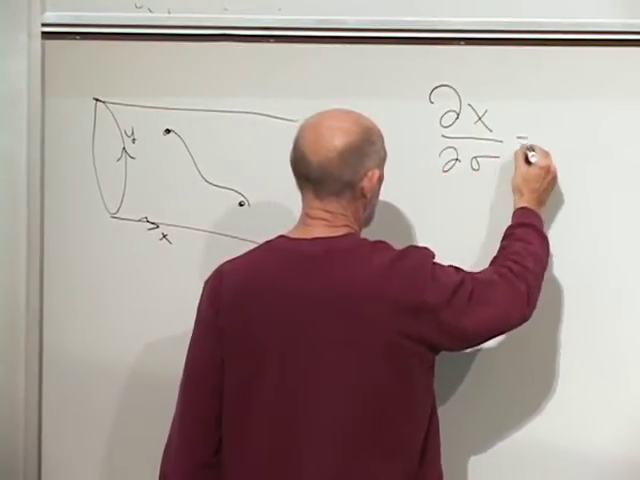
\includegraphics[width=\linewidth]{lecture_10_figure_05.png}
    \par\smallskip
    \textit{Bán kính compact lớn.}
  \end{minipage}\hfill
  \begin{minipage}[t]{0.48\textwidth}
    \centering
    \includegraphics[width=\linewidth]{lecture_10_figure_06.png}
    \par\smallskip
    \textit{Bán kính compact nhỏ.}
  \end{minipage}
  \caption{Hai phép so sánh phổ trên bảng. Các tháp mức thưa và dày đổi vai trò cho nhau khi bán kính được lấy nghịch đảo của nó.}
  \lectureframe{00:25:30--00:26:00}
  \label{fig:l10-dual-spectra-board}
\end{figure}

Sơ đồ gọn nhất là
\begin{figure}[H]
  \centering
  \begin{adjustbox}{max width=\linewidth}
  \begin{tikzpicture}[x=1cm,y=0.74cm,>=Latex]
    \node[font=\bfseries] at (-3.6,6.2) {$R\gg\sqrt{\alpha'}$};
    \draw[->] (-5.1,0) -- (-5.1,5.5) node[above] {$E$};
    \foreach \y in {0.4,1.0,1.6,2.2,2.8,3.4,4.0,4.6}
      \draw (-5.35,\y)--(-4.85,\y);
    \node[align=center] at (-4.25,5.15) {momentum\\dense};
    \draw[->] (-2.2,0) -- (-2.2,5.5) node[above] {$E$};
    \foreach \y in {0.4,2.4,4.4}
      \draw (-2.45,\y)--(-1.95,\y);
    \node[align=center] at (-1.35,5.15) {winding\\sparse};

    \node[font=\bfseries] at (3.6,6.2) {$R\ll\sqrt{\alpha'}$};
    \draw[->] (2.2,0) -- (2.2,5.5) node[above] {$E$};
    \foreach \y in {0.4,2.4,4.4}
      \draw (1.95,\y)--(2.45,\y);
    \node[align=center] at (3.05,5.15) {momentum\\sparse};
    \draw[->] (5.1,0) -- (5.1,5.5) node[above] {$E$};
    \foreach \y in {0.4,1.0,1.6,2.2,2.8,3.4,4.0,4.6}
      \draw (4.85,\y)--(5.35,\y);
    \node[align=center] at (5.95,5.15) {winding\\dense};
  \end{tikzpicture}
  \end{adjustbox}
  \caption{Bản dựng lại của lập luận về khoảng cách mức. Phổ dây đầy đủ không đổi khi hoán đổi xung lượng và số quấn đồng thời với \(R\leftrightarrow\alpha'/R\).}
  \label{fig:l10-dual-spectra-redraw}
\end{figure}

Giả sử một quan sát viên được đưa cho một trong các phổ này mà không được nói nó được tạo ra thế nào. Tháp mức sít nhau là xung lượng trên một đường tròn lớn, hay là quấn trên một đường tròn nhỏ? Chỉ riêng phổ không thể cho biết. Lý thuyết dây đưa ra phát biểu mạnh hơn rằng biên độ tán xạ cũng không thể cho biết. Hai mô tả hoàn toàn tương đương dưới
\begin{equation}
  n\longleftrightarrow w,
  \qquad
  R\longleftrightarrow \widetilde R=\frac{\alpha'}{R}.
  \label{eq:l10-radius-duality}
\end{equation}
Điểm bất động là
\begin{equation}
  R=\sqrt{\alpha'},
  \label{eq:l10-self-dual-radius}
\end{equation}
hay \(R=1\) trong đơn vị của bài giảng. Tại bán kính đó, các trạng thái bổ sung có thể trở nên không khối lượng và đối xứng chuẩn được tăng cường.

\begin{classroomqa}
\audiencequestion{Số quấn có chỉ là một tiện ích toán học để viết lại phổ không? \lecturetimestamp{00:27:33}}
\lecturerresponse{Không. Số quấn gắn nhãn những sector thực của không gian Hilbert dây kín, và những sector đó tham gia vào các tương tác. Từ ``đối ngẫu'' có nghĩa là mô tả xung lượng và mô tả số quấn là hai hệ tọa độ khác nhau của cùng một vật lý, chứ không phải rằng một sector chỉ là một mẹo ghi nhớ tùy chọn cho sector kia.}
\end{classroomqa}

\begin{classroomqa}
\audiencequestion{Có bán kính nào được ánh xạ vào chính nó không?
\lecturetimestamp{00:27:58}}
\lecturerresponse{Có. Giá trị tự đối ngẫu là \(R=\sqrt{\alpha'}\), tức là \(R=1\) trong các đơn vị dùng trên bảng. Hai tháp mức gặp nhau tại đó, và phổ có đối xứng được tăng cường.}
\end{classroomqa}

\section{Dạng worldsheet của đối ngẫu}

Lập luận phổ là gợi ý tốt, nhưng worldsheet làm cho sự hoán đổi trở nên chính xác hơn. Trong chuẩn chỉnh hình, xung lượng liên hợp với \(Y\) tỉ lệ với \(\partial_\tau Y\). Vì vậy tổng xung lượng theo phương compact có dạng
\begin{equation}
  P_Y=\frac{1}{2\pi\alpha'}
      \int_0^{2\pi}d\sigma\,\partial_\tau Y.
  \label{eq:l10-worldsheet-momentum}
\end{equation}
Số quấn là
\begin{equation}
  w=\frac{1}{2\pi R}
      \int_0^{2\pi}d\sigma\,\partial_\sigma Y
   =\frac{Y(2\pi)-Y(0)}{2\pi R}.
  \label{eq:l10-worldsheet-winding}
\end{equation}

\begin{classroomqa}
\audiencequestion{Vì sao tích phân của một đạo hàm lại không triệt tiêu quanh dây kín? \lecturetimestamp{00:32:33}}
\lecturerresponse{Vì \(Y\) là một tọa độ tuần hoàn của không gian đích, chứ không phải một hàm thực đơn trị trên đường tròn \(\sigma\). Điểm worldsheet \(\sigma=2\pi\) là cùng một điểm với \(\sigma=0\), nhưng một phép nâng của phép nhúng lên đường thẳng phủ thay đổi một lượng \(2\pi wR\). Tích phân của \(\partial_\sigma Y\) đo độ dịch đó.}
\end{classroomqa}

\begin{figure}[H]
  \centering
  \includegraphics[width=0.76\textwidth]{lecture_10_figure_07.png}
  \caption{Các tích phân của xung lượng và số quấn sau khi cả hai dòng đã được hoàn tất trên bảng. Các thừa số chung \(2\pi\) và \(\alpha'\) bị lược bỏ trong chuẩn hóa của bài giảng.}
  \lectureframe{00:33:25}
  \label{fig:l10-momentum-winding-integrals}
\end{figure}

Đối với một dây quấn một vòng,
\begin{equation}
  Y(\tau,\sigma+2\pi)=Y(\tau,\sigma)+2\pi R.
\end{equation}
Với số quấn \(w\), độ dịch ở vế phải là \(2\pi wR\). Khi đó phương trình \eqref{eq:l10-worldsheet-winding} đếm chính xác số quấn. Đây là phiên bản chính xác của lối viết tắt trên bảng \(w\sim R^{-1}\int
d\sigma\,\partial_\sigma Y\).

Vì vậy, phát biểu trên worldsheet của đối ngẫu T là
\begin{equation}
  \partial_\tau Y\longleftrightarrow
  \partial_\sigma \widetilde Y,
  \qquad
  \partial_\sigma Y\longleftrightarrow
  \partial_\tau \widetilde Y,
  \label{eq:l10-derivative-duality}
\end{equation}
trong đó xung lượng theo \(Y\) trở thành số quấn trong tọa độ đối ngẫu \(\widetilde Y\), và ngược lại.

\begin{classroomqa}
\audiencequestion{Điều này có nghĩa là bản thân các tọa độ worldsheet \(\tau\) và \(\sigma\) có liên hệ với nhau hay bị hoán đổi cho nhau không?
\lecturetimestamp{00:34:39}}
\lecturerresponse{Không. Đối ngẫu T ánh xạ các nghiệm và hoán đổi những đạo hàm nhất định của tọa độ đích compact. Nó không đồng nhất tọa độ thời gian của worldsheet với tọa độ không gian của worldsheet.}
\end{classroomqa}

\section{Vì sao không thể tránh các trạng thái quấn}

Người ta có thể hỏi vì sao một dây lại có thể được thấy ở trạng thái có quấn khi vẫn có sẵn một trạng thái không quấn. Một dây không chọn trạng thái của nó theo sở thích. Năng lượng được cung cấp trong một va chạm sẽ kéo dãn nó. Một dây đủ năng lượng và bị méo mạnh có thể tái nối thành hai dây có số quấn đối nhau. Tổng số quấn của chúng vẫn bằng không, nhưng sau khi tách ra hai dây có thể rời xa nhau. Một thành viên của cặp có thể bị đưa đi rất xa, để lại cho một quan sát viên một dây có quấn dường như cô lập.

\begin{figure}[H]
  \centering
  \includegraphics[width=0.76\textwidth]{lecture_10_figure_08.png}
  \caption{Một cấu hình có tổng số quấn bằng không nhưng bị kéo dãn mạnh, từ đó các dây có số quấn đối nhau có thể tách ra sau khi tái nối.}
  \lectureframe{00:36:15}
  \label{fig:l10-winding-pair-production}
\end{figure}

Ngưỡng năng lượng được đặt bởi năng lượng quấn. Trên một đường tròn lớn, cần một năng lượng va chạm lớn để kéo đủ chiều dài dây quanh phương compact. Tuy nhiên, một khi vượt ngưỡng, sự tạo cặp quấn--phản quấn không thể bị cấm. Phép tương tự là va chạm photon tạo ra một cặp electron--positron. Tổng điện tích vẫn bằng không, nhưng các hạt mang điện vẫn có mặt và có thể bị tách ra. Bảo toàn số quấn vận hành theo đúng cách đó.

Phép loại suy này không chỉ là bằng lời. Động lượng compact và số quấn hành xử như hai số lượng tử điện tích khác biệt. Trong mô tả rút gọn tương ứng, cùng dấu đẩy nhau và trái dấu hút nhau. Vì vậy, ta nên hỏi hai trường vectơ nào làm trung gian cho các lực đó.

\section{Điện tích động lượng từ hấp dẫn năm chiều}

Hãy bắt đầu với hấp dẫn trong năm chiều. Cho các chỉ số hoa \(M,N\) chạy trên bốn phương không-thời gian thông thường và chiều thứ năm compact. Metric phân rã thành
\begin{equation}
  G_{MN}\quad\longrightarrow\quad
  \bigl\{G_{\mu\nu},\,G_{\mu5},\,G_{55}\bigr\}.
  \label{eq:l10-metric-decomposition}
\end{equation}
Thành phần đối xứng \(G_{5\mu}\) không chứa thông tin mới nào ngoài \(G_{\mu5}\).

\begin{figure}[H]
  \centering
  \includegraphics[width=0.74\textwidth]{lecture_10_figure_09.png}
  \caption{Các nhóm độc lập của các thành phần metric năm chiều: \(G_{\mu\nu}\), \(G_{\mu5}\) và \(G_{55}\).}
  \lectureframe{00:44:05}
  \label{fig:l10-metric-components}
\end{figure}

Từ quan điểm bốn chiều,
\begin{align}
  G_{\mu\nu} &\quad\hbox{is a spacetime metric},\\
  G_{\mu5} &\equiv A_\mu\quad\hbox{is a vector field},\\
  G_{55} &\equiv e^{2\varphi}\quad\hbox{is a scalar modulus}.
  \label{eq:l10-four-dimensional-fields}
\end{align}
Vô hướng \(\varphi\) đo kích thước của chiều compact. Nó có thể biến thiên trơn trên không-thời gian thông thường, nên các sóng của \(\varphi\) là các sóng của bán kính chiều thứ năm.

\begin{figure}[H]
  \centering
  \includegraphics[width=0.74\textwidth]{lecture_10_figure_10.png}
  \caption{Trên bảng, \(G_{\mu5}\) được đồng nhất với một vectơ \(A_\mu\), còn \(G_{55}\) với một vô hướng \(\Phi\).}
  \lectureframe{00:47:40}
  \label{fig:l10-vector-and-radius-modulus}
\end{figure}

Nguồn của một thành phần hấp dẫn hỗn hợp là dòng động lượng hỗn hợp. Cụ thể, động lượng theo chiều thứ năm là nguồn của \(G_{\mu5}\). Vì vậy, một quan sát viên bốn chiều diễn giải số nguyên \(n\) như một điện tích ghép với \(A_\mu\). Đây là cơ chế Kaluza--Klein: cái là động lượng trong hình học số chiều cao hơn trở thành điện tích trong lý thuyết trường số chiều thấp hơn.

\editorialnote{Bài giảng gọi một cách không chặt chẽ vô hướng xuất phát từ \(G_{55}\) là một ``dilaton''. Trong phép rút gọn này, nó cụ thể là môđun bán kính. Dilaton dây mười chiều, trường chi phối hằng số ghép dây, là một trường riêng biệt, mặc dù các tổ hợp vô hướng ở số chiều thấp hơn có thể trộn lẫn dưới các phép đổi khung và đối ngẫu.}

\begin{classroomqa}
\audiencequestion{Vô hướng \(\varphi\) có tỉ lệ với số nguyên động lượng \(n\) không? \lecturetimestamp{00:48:43}}
\lecturerresponse{Không. Số nguyên \(n\) gắn nhãn một trạng thái lượng tử hóa và đóng vai trò điện tích. Vô hướng \(\varphi(x)\) là một trường liên tục quyết định kích thước compact hóa địa phương. Nó có thể thay đổi từ nơi này sang nơi khác; bản thân nó không phải là một số nguyên.}
\end{classroomqa}

\section{Trường vectơ thứ hai và điện tích số quấn}

Số quấn cũng mang tính điện tích, nhưng nó không thể ghép với cùng một vectơ theo cùng cách đó. Để thấy vectơ thứ hai, hãy quay lại các kích thích đầu tiên của dây kín. Một dây kín có các mode dao động tử chuyển trái và chuyển phải. Các trạng thái vật lý tuân theo điều kiện khớp mức: tổng các mức kích thích trái và phải phải bằng nhau.

Trong lý thuyết boson, trạng thái không kích thích là tachyon. Một dao động tử chuyển trái hoặc chuyển phải đơn lẻ sẽ vi phạm điều kiện khớp mức. Vì vậy, trạng thái không khối lượng đầu tiên được phép chứa một dao động tử của mỗi loại,
\begin{equation}
  \alpha_{-1}^{I}\widetilde\alpha_{-1}^{J}\ket{0;k}.
  \label{eq:l10-first-massless-state}
\end{equation}
Các chỉ số \(I,J\) chạy trên các phương không gian ngang, kể cả chiều compact. Nếu một chỉ số là thông thường còn chỉ số kia là \(5\), thì có hai trạng thái dao động tử kiểu vectơ,
\begin{equation}
  \alpha_{-1}^{\mu}\widetilde\alpha_{-1}^{5}\ket{0;k},
  \qquad
  \alpha_{-1}^{5}\widetilde\alpha_{-1}^{\mu}\ket{0;k}.
  \label{eq:l10-two-vector-states}
\end{equation}

\begin{figure}[H]
  \centering
  \includegraphics[width=0.76\textwidth]{lecture_10_figure_11.png}
  \caption{Hai thứ tự dao động tử trái--phải trở thành các trạng thái vectơ bốn chiều khi một phân cực hướng dọc theo chiều compact.}
  \lectureframe{00:58:20}
  \label{fig:l10-two-vector-states-board}
\end{figure}

Các tổ hợp đối xứng và phản đối xứng của chúng thuộc về các trường không-thời gian khác nhau:
\begin{align}
  \alpha_{-1}^{(\mu}\widetilde\alpha_{-1}^{5)}\ket{0;k}
    &\longleftrightarrow G_{\mu5},\\
  \alpha_{-1}^{[\mu}\widetilde\alpha_{-1}^{5]}\ket{0;k}
    &\longleftrightarrow B_{\mu5}.
  \label{eq:l10-g-and-b-vectors}
\end{align}
Trường thứ nhất là vectơ Kaluza--Klein do động lượng compact làm nguồn. Trường thứ hai đi xuống từ trường phản đối xứng Kalb--Ramond và do số quấn của dây làm nguồn. Vì thế, lý thuyết rút gọn chứa hai trường kiểu photon, một cho mỗi loại điện tích.

Nếu cả hai chỉ số dao động tử đều hướng dọc theo chiều compact, thì trạng thái đó là một vô hướng gắn với môđun compact hóa. Nếu cả hai đều nằm trong các phương ngang thông thường, thì phần đối xứng không vết là graviton, phần phản đối xứng là \(B_{\mu\nu}\), và phần vết đóng góp vào một sector vô hướng.

\begin{classroomqa}
\audiencequestion{Trong các trạng thái này, trạng thái nào là singlet và trạng thái nào là triplet? \lecturetimestamp{01:00:21}}
\lecturerresponse{Cách phân loại đó không hữu ích ở đây. Cả hai trạng thái hỗn hợp đều biến đổi như các vectơ bốn chiều. Tổng và hiệu của chúng tách phân cực metric đối xứng khỏi phân cực trường \(B\) phản đối xứng. Trạng thái có hai chỉ số compact thay vào đó là một vô hướng bốn chiều.}
\end{classroomqa}

Bảng đối chiếu đầy đủ thu được trước giờ nghỉ là
\begin{equation}
  \boxed{
  \begin{gathered}
    n\leftrightarrow w,
    \qquad
    R\leftrightarrow\dfrac{\alpha'}{R},\\
    \partial_\tau Y\leftrightarrow\partial_\sigma\widetilde Y,
    \qquad
    G_{\mu5}\leftrightarrow B_{\mu5}.
  \end{gathered}}
  \label{eq:l10-complete-t-duality-map}
\end{equation}

\begin{figure}[H]
  \centering
  \includegraphics[width=0.72\textwidth]{lecture_10_figure_12.png}
  \caption{Bản tóm tắt trên bảng về ánh xạ đối ngẫu T: động lượng và số quấn, bán kính và bán kính nghịch đảo, các đạo hàm trên mặt thế giới, và hai trường vectơ được hoán đổi cho nhau. Giảng viên che khuất một phần dòng cuối, nên dòng đó được bổ sung tường minh trong Phương trình
  \eqref{eq:l10-complete-t-duality-map}.}
  \lectureframe{01:02:20}
  \label{fig:l10-t-duality-map-board}
\end{figure}

Không nên nhầm cách xây dựng này với khẳng định rằng mọi trường vừa liệt kê đều đã được nhận diện trong phổ hạt quan sát được. Ở đây, nó là một hệ quả toán học của lý thuyết dây đã compact hóa. Có nhiều đề xuất nhằm nối những cấu trúc như vậy với hiện tượng học, nhưng đó không phải là bài toán đang được giải trong bài giảng này.

\section{Dây mở làm thay đổi câu hỏi}

Sau giờ nghỉ, ta bắt đầu lại với dây mở. Một dây kín có thể có số quấn bền vì nó không có đầu mút để số quấn có thể tuột mất. Dây mở có các đầu mút nên không có số quấn được bảo vệ tôpô tương tự. Tuy vậy, đối ngẫu T là một đối xứng chính xác của lý thuyết. Đối xứng ấy tác động lên dây mở như thế nào?

Đối với một đầu mút chuyển động tự do, phép biến phân của tác dụng dây cho ra điều kiện biên Neumann. Trong hình học đơn giản \((X,Y)\),
\begin{equation}
  \left.\partial_\sigma X\right|_{\partial\Sigma}=0,
  \qquad
  \left.\partial_\sigma Y\right|_{\partial\Sigma}=0.
  \label{eq:l10-neumann-boundary}
\end{equation}
Bức tranh cơ học thì đơn giản. Hãy xem dây như một chuỗi các phần tử khối lượng ngày càng nhỏ. Một lực tiếp tuyến khác không tác dụng lên phần tử cuối cùng sẽ gây cho nó một gia tốc phân kỳ khi khối lượng của nó tiến tới 0. Vì vậy, một đầu mút tự do sẽ tự điều chỉnh cho tới khi lực căng tổng tại đầu mút triệt tiêu. Dĩ nhiên, ai đó có thể giữ cố định đầu mút và cung cấp lực cần thiết, nhưng khi ấy đầu mút sẽ không còn tự do nữa.

\begin{figure}[H]
  \centering
  \includegraphics[width=0.76\textwidth]{lecture_10_figure_13.png}
  \caption{Dây mở và các điều kiện Neumann tại đầu mút đầy đủ của nó, \(\partial_\sigma X=\partial_\sigma Y=0\).}
  \lectureframe{01:09:20}
  \label{fig:l10-neumann-board}
\end{figure}

Bây giờ chỉ đối ngẫu hóa tọa độ compact \(Y\). Tọa độ không compact \(X\) không đổi. Phương trình \eqref{eq:l10-derivative-duality} biến điều kiện Neumann thứ hai thành
\begin{equation}
  \left.\partial_\tau\widetilde Y\right|_{\partial\Sigma}=0.
  \label{eq:l10-dirichlet-time-derivative}
\end{equation}
Vì vậy, đầu mút có vị trí không đổi theo thời gian trong chiều compact đối ngẫu,
\begin{equation}
  \left.\widetilde Y\right|_{\partial\Sigma}=Y_0.
  \label{eq:l10-dirichlet-boundary}
\end{equation}
Đây là một điều kiện biên Dirichlet.

\begin{figure}[H]
  \centering
  \includegraphics[width=0.76\textwidth]{lecture_10_figure_14.png}
  \medskip

  \begin{adjustbox}{max width=\linewidth}
  \begin{tikzpicture}[x=1cm,y=1cm,>=Latex]
    \node[align=center] at (-3.5,0.8)
      {Neumann\\\(\left.\partial_\sigma Y\right|_{\partial\Sigma}=0\)};
    \draw[->,thick] (-1.7,0.8) -- (1.3,0.8)
      node[midway,above] {$T_Y$};
    \node[align=center] at (3.4,0.8)
      {Dirichlet\\\(\left.\partial_\tau\widetilde Y\right|_{\partial\Sigma}=0\)};
    \node[align=center] at (3.4,-0.5)
      {\(\widetilde Y(\tau)=Y_0\) at each endpoint};
  \end{tikzpicture}
  \end{adjustbox}
  \caption{Điều kiện đầu mút đối ngẫu hoàn chỉnh trên bảng và sự tái dựng logic rõ ràng của nó. Đối ngẫu T biến sự tự do trong chiều compact thành một vị trí đầu mút cố định trong chiều đối ngẫu.}
  \lectureframe{01:12:35}
  \label{fig:l10-neumann-to-dirichlet}
\end{figure}

\begin{classroomqa}
\audiencequestion{Vì sao điều kiện đối ngẫu lại có nghĩa là đầu mút bị cố định? \lecturetimestamp{01:12:39}}
\lecturerresponse{Vì \(\partial_\tau\widetilde Y=0\) có nghĩa là vận tốc bằng 0 theo chiều đã đối ngẫu hóa. Đầu mút bắt đầu ở đâu trong \(\widetilde Y\) thì nó sẽ ở nguyên tại đó. Các tọa độ của nó song song với các phương chưa đối ngẫu hóa vẫn tự do.}
\end{classroomqa}

\section{Vật giữ đầu mút là một D-brane}

Nếu một đầu mút bị cố định, thì phải có cái gì đó giữ được nó tại chỗ. Vì vậy, đối ngẫu T chính xác đòi hỏi một đối tượng mới mà trên đó dây mở có thể tận cùng. Đối tượng ấy là một D-brane. Chữ \(D\) là viết tắt của Dirichlet, không phải của số chiều của đối tượng. Trong phần bình luận lịch sử ngắn của bài giảng, người ta hẳn đã có thể đặt tên các đối tượng này theo Joseph Polchinski, người mà phân tích của ông đã làm cho vai trò động lực học của chúng trở nên hiển nhiên, nhưng thuật ngữ đã có sẵn ``p-brane'' khiến Dirichlet trở thành tên gọi tự nhiên.

Một \(p\)-brane có \(p\) chiều không gian. Dây là một one-brane, màng là một two-brane, và một vật thể kéo dài ba chiều là một three-brane. Một D\(p\)-brane là một \(p\)-brane mà trên đó các đầu mút của dây cơ bản tuân theo điều kiện Dirichlet trong các phương ngang và điều kiện Neumann trong các phương tiếp tuyến với brane.

Không có gì trong lập luận đối ngẫu chọn riêng một giá trị nào của \(Y_0\), nên D-brane không thể là một vật cố định cứng bị đóng đinh tại một điểm ưu tiên nào đó trong vũ trụ. Nó phải có thể di chuyển được. Thuyết tương đối cũng cấm một vật thể kéo dài tuyệt đối cứng, nên một D-brane có thể dao động và uốn cong. Brane phẳng đơn giản được vẽ trên bảng là cấu hình cân bằng của nó, không phải một sự hạn chế đối với động lực học của nó.

\begin{classroomqa}
\audiencequestion{Hai đầu mút của một dây mở có nhất thiết phải có cùng một giá trị cố định của tọa độ đối ngẫu không? \lecturetimestamp{01:14:55}}
\lecturerresponse{Nói chung là không. Cả hai đầu mút có thể nằm trên cùng một D-brane, trong trường hợp đó chúng chia sẻ cùng vị trí ngang của brane ấy. Chúng cũng có thể nằm trên hai D-brane khác nhau ở các vị trí ngang khác nhau, và khi đó dây sẽ căng giữa chúng. Bản thân brane cũng có thể dao động và uốn cong, nên quỹ tích đầu mút không nhất thiết phải luôn là một mặt phẳng hoàn toàn phẳng.}
\end{classroomqa}

\section{Đếm số chiều của một D-brane}

Lý thuyết siêu dây mười chiều có chín chiều không gian. Giả sử đối ngẫu T áp đặt một điều kiện Dirichlet theo một phương không gian. Đầu mút vẫn tự do trong tám phương còn lại, nên quỹ tích được phép của nó là một D8-brane tám chiều. Mỗi điều kiện Dirichlet độc lập bổ sung loại bỏ một phương chuyển động của đầu mút. Nếu \(k\) tọa độ không gian bị cố định, thì
\begin{equation}
  p=9-k.
  \label{eq:l10-dp-counting}
\end{equation}

Ví dụ mặt bàn cho phiên bản ba chiều của cùng phép đếm ấy. Cố định tọa độ thẳng đứng thì đầu ngón tay có thể di chuyển trên một mặt bàn hai chiều. Cố định thêm tọa độ thứ hai thì nó chỉ có thể di chuyển dọc theo một đường thẳng. Cố định cả ba thì nó bị giam tại một điểm.

\begin{figure}[H]
  \centering
  \begin{adjustbox}{max width=\linewidth}
  \begin{tikzpicture}[x=1.05cm,y=1cm,>=Latex]
    \draw[fill=blue!8] (-5.5,-0.7) -- (-2.5,-0.7) -- (-1.7,0.2)
      -- (-4.7,0.2) -- cycle;
    \node at (-3.6,-1.15) {one constraint: sheet};
    \draw[very thick,blue!60!black] (-0.9,-0.25) -- (1.3,-0.25);
    \node at (0.2,-1.15) {two constraints: line};
    \fill[blue!70!black] (4.1,-0.25) circle (0.09);
    \node at (4.1,-1.15) {three constraints: point};
    \draw[->] (-1.45,0.95) -- (-0.75,0.95);
    \draw[->] (2.25,0.95) -- (2.95,0.95);
    \node at (0.35,1.35) {each Dirichlet condition lowers \(p\) by one};
  \end{tikzpicture}
  \end{adjustbox}
  \caption{Lập luận đếm số chiều được dùng trong ví dụ mặt bàn. Một D\(p\)-brane là quỹ tích trong đó các đầu mút vẫn tự do chuyển động.}
  \label{fig:l10-dp-counting-redraw}
\end{figure}

Các phép đối ngẫu lặp lại sinh ra các D8-, D7-, D6-brane, v.v., cho tới một D0-brane, là một đối tượng dạng điểm trong không gian. Nếu không có phương không gian nào bị cố định, thì một D9-brane chiếm trọn cả chín chiều không gian và các dây mở thông thường tự do di chuyển khắp nơi. Bài giảng có nhắc ngắn gọn đến các D\((-1)\)-brane; chúng khu trú trong không-thời gian Euclid và hành xử như instanton hơn là như các hạt thông thường lan truyền theo thời gian.

\editorialnote{Bậc thang số chiều là một phát biểu về hai lý thuyết loại II khi xét chung. Các D\(p\)-brane BPS bền có \(p\) chẵn trong type IIA và \(p\) lẻ trong type IIB. Đối ngẫu T dọc theo một đường tròn làm thay đổi \(p\) đi một đơn vị và đồng thời trao đổi type IIA với type IIB.}

\begin{classroomqa}
\audiencequestion{Nếu chỉ có sáu chiều là compact, thì phép đếm có nên bắt đầu bằng cách trừ từ sáu thay vì từ chín không? \lecturetimestamp{01:20:49}}
\lecturerresponse{Phép suy ra sơ cấp thực hiện đối ngẫu T trên các phương compact, nhưng một đường tròn đối ngẫu trở nên lớn tùy ý khi đường tròn ban đầu trở nên nhỏ tùy ý. Trong giới hạn đó, nó hiệu dụng là không compact. Vì thế, các brane thu được có thể kéo dài dọc theo hoặc vuông góc với những phương mà ở các thang đo có thể tiếp cận trông như không compact. Số chiều \(p\) đếm tất cả các phương không gian tiếp tuyến với brane, chứ không chỉ các phương compact được dùng trong một phép suy ra.}
\end{classroomqa}

Một D0-brane là một loại hạt mới. Một dây mở có thể nối từ một D0-brane sang một brane khác, quay về chính D0-brane đó, hoặc kéo dài về phía một brane ở rất xa. Nếu hiểu theo nghĩa đen là kéo ra vô cực không gian thì một dây có độ dài vô hạn và do đó năng lượng vô hạn, vì vậy phiên bản hữu ích về mặt vật lý đặt đầu mút còn lại của nó trên một đối tượng khác.

Trường hợp tiếp theo, D1-brane, bản thân nó có dạng sợi dây, nhưng không phải là dây cơ bản mà ta đã bắt đầu với. Nó có thể uốn cong và khép lại trên chính nó, và các dây cơ bản có thể kết thúc trên nó. Sức căng của nó biến thiên theo hằng số liên kết dây theo một cách khác:
\begin{equation}
  T_{\rm D1}=\frac{1}{2\pi\alpha' g_s},
  \qquad
  T_{\rm F1}=\frac{1}{2\pi\alpha'}.
  \label{eq:l10-dstring-tension}
\end{equation}
Ở chế độ liên kết yếu \(g_s\ll1\), D-dây nặng hơn nhiều so với dây cơ bản, điều này giải thích vì sao ban đầu nó xuất hiện như một điểm neo có khối lượng lớn.

\begin{figure}[H]
  \centering
  \includegraphics[width=0.76\textwidth]{lecture_10_figure_15.png}
  \caption{D1-brane trên bảng: một đối tượng một chiều có thể uốn cong, khác với các dây cơ bản có thể kết thúc trên nó.}
  \lectureframe{01:24:20}
  \label{fig:l10-d1-brane}
\end{figure}

\begin{classroomqa}
\audiencequestion{Đối ngẫu T có tác động lên các D-brane cũng như lên các dây không? \lecturetimestamp{01:25:35}}
\lecturerresponse{Có. Một phép đối ngẫu T theo một phương song song với một D\(p\)-brane làm hạ số chiều của nó xuống D\((p-1)\), còn một phép đối ngẫu T theo một phương trực giao với nó làm tăng số chiều lên D\((p+1)\). Các brane là một phần của từ điển đối ngẫu, chứ không phải những giá đỡ bên ngoài vẫn giữ nguyên dưới phép đó.}
\end{classroomqa}

\begin{classroomqa}
\audiencequestion{Các phương tiếp tuyến với một brane vẫn có thể là compact chứ?
\lecturetimestamp{01:27:25}}
\lecturerresponse{Có. ``Tiếp tuyến'' và ``compact'' trả lời những câu hỏi khác nhau. Một phương có thể nằm dọc theo brane mà vẫn khép thành một đường tròn; nó cũng có thể là không compact. Điều quan trọng đối với đầu mút là điều kiện biên theo phương đó là Neumann hay Dirichlet.}
\end{classroomqa}

Một D2-brane là một tấm dạng màng. Một D3-brane có ba chiều không gian. Trong một không-thời gian thực sự nhiều chiều hơn, một D3-brane là một không gian con ba chiều chứ không phải toàn bộ không gian, mặc dù những quan sát viên bị giới hạn trên nó có thể trải nghiệm nó như toàn bộ thế giới không gian của mình.

\begin{figure}[H]
  \centering
  \includegraphics[width=0.76\textwidth]{lecture_10_figure_16.png}
  \caption{Một D2-brane được vẽ như một tấm mà trên đó các đầu mút dây có thể chuyển động.}
  \lectureframe{01:27:55}
  \label{fig:l10-d2-brane}
\end{figure}

Phép suy ra trình bày ở đây cố ý chỉ là một phác thảo. Tự nó không phải là bằng chứng rằng lý thuyết dây mô tả tự nhiên. Tuy nhiên, bên trong lý thuyết dây, các kiểm tra nhất quán là rất nhiều: các đối ngẫu, các tính toán lượng tử và các kết quả toán học đều chỉ ra rằng D-brane là những đối tượng động lực học đích thực.

\section{Các dây mở trở thành các trường trên một brane}

Hãy lấy một D2-brane vốn trống và đặt lên nó các dây mở ngắn. Mỗi đầu mút bị giới hạn trên tấm đó, nên toàn bộ kích thích năng lượng thấp chuyển động dọc theo tấm. Hai dây có định hướng mà các đầu mút kề nhau mang các mũi tên tương thích có thể nối lại. Dây đã nối về sau có thể lại tách ra. Nếu đọc như lịch sử của các hạt, thì đây là các đỉnh của giản đồ Feynman: hai hạt đi vào, một kích thích trung gian lan truyền, và hai hạt đi ra.

\begin{figure}[H]
  \centering
  \includegraphics[width=0.76\textwidth]{lecture_10_figure_17.png}
  \caption{Các dây mở có định hướng trên một D2-brane nối với nhau qua các đầu mút tương thích. Ở năng lượng thấp, quá trình này được hiểu như một tương tác lý thuyết trường trên brane.}
  \lectureframe{01:29:55}
  \label{fig:l10-open-strings-on-brane}
\end{figure}

Ở các năng lượng thấp hơn nhiều so với thang dây, tháp các mode dao động nội tại không được kích thích. Trạng thái dây mở không khối lượng còn lại là một trường vectơ trên thể tích thế giới của brane. Với một brane, đó là một trường chuẩn abel \(U(1)\), tương tự điện từ học trên brane. Trường ấy không lan truyền trong toàn bộ không gian khối mười chiều; các lượng tử của nó là những dây mở mà các đầu mút giữ chúng trên brane.

\section{Một chồng brane tạo ra màu không abel}

Bây giờ hãy đặt vài brane song song ở gần nhau. Với ba brane, hãy gán nhãn chúng là Red, Green và Blue. Một dây có định hướng mang một cặp có thứ tự gồm các nhãn đầu mút: nó có thể đi từ Red đến Green, từ Green đến Blue, từ Red đến Red, v.v. Với \(N\) brane, các trạng thái dây mở không khối lượng có thể được sắp thành một ma trận \(N\times N\)
\begin{equation}
  A_\mu{}^{i}{}_{j},
  \qquad i,j=1,\ldots,N.
  \label{eq:l10-chan-paton-matrix}
\end{equation}
Đó là các nhãn Chan--Paton của một lý thuyết chuẩn \(U(N)\).

\begin{figure}[H]
  \centering
  \includegraphics[width=0.76\textwidth]{lecture_10_figure_18.png}
  \medskip

  \begin{adjustbox}{max width=\linewidth}
  \begin{tikzpicture}[x=1cm,y=1cm,>=Latex]
    \draw[very thick,red!70!black] (-4.8,2.0)--(4.8,2.0);
    \draw[very thick,green!55!black] (-4.8,0.8)--(4.8,0.8);
    \draw[very thick,blue!70!black] (-4.8,-0.4)--(4.8,-0.4);
    \node[left] at (-4.8,2.0) {Red};
    \node[left] at (-4.8,0.8) {Green};
    \node[left] at (-4.8,-0.4) {Blue};
    \draw[->,thick] (-3.4,2.0) .. controls (-2.8,1.35) and (-2.3,1.15)
      .. (-1.7,0.8);
    \node at (-2.7,1.05) {$R\!G$};
    \draw[->,thick] (-0.6,0.8) .. controls (0.0,0.25) and (0.6,-0.05)
      .. (1.2,-0.4);
    \node at (0.1,0.0) {$G\!B$};
    \draw[->,thick] (2.1,2.0) .. controls (2.9,2.55) and (3.8,2.55)
      .. (4.3,2.0);
    \node at (3.2,2.65) {$R\!R$};
  \end{tikzpicture}
  \end{adjustbox}
  \caption{Ba brane song song trên bảng và cách dựng lại rõ ràng các nhãn đầu mút có thứ tự do những dây giữa chúng mang.}
  \lectureframe{01:33:15}
  \label{fig:l10-three-brane-stack}
\end{figure}

\begin{classroomqa}
\audiencequestion{Một dây có thật sự thể chạy từ brane Red đến brane Green mà không bị các hình vẽ khác chặn lại không? \lecturetimestamp{01:35:07}}
\lecturerresponse{Có. Các brane được nhúng trong một không gian nhiều chiều hơn. Hình vẽ hai chiều trên bảng chỉ là một phép chiếu, nên một dây có thể đi vòng qua một đường được chiếu khác theo một phương trực giao.}
\end{classroomqa}

\begin{classroomqa}
\audiencequestion{Một dây Red--Green có bắt buộc phải ghép với một dây Green--Blue để trở thành Red--Blue không? \lecturetimestamp{01:35:39}}
\lecturerresponse{Đó là quy tắc nối cục bộ cơ bản. Các đầu mút tương thích gặp nhau, và hai đoạn trở thành một dây duy nhất mà các đầu mút chưa nối của nó giữ lại các nhãn Red và Blue. Những quá trình phức tạp hơn được xây dựng bằng cách lặp lại cùng phép đó.}
\end{classroomqa}

Quy tắc nối là phép nhân ma trận được hình học hóa. Một dây Red--Green có thể nối với một dây Green--Blue vì đầu mút Green của cái này tương thích với đầu mút Green của cái kia. Kết quả là một dây Red--Blue:
\begin{equation}
  (R,G)\circ(G,B)\longrightarrow(R,B).
  \label{eq:l10-color-composition}
\end{equation}
Chỉ số lặp được nối lại và biến mất ở bên trong. Đây chính là cùng một cấu trúc chỉ số xuất hiện tại một đỉnh tương tác Yang--Mills.

\begin{figure}[H]
  \centering
  \includegraphics[width=0.76\textwidth]{lecture_10_figure_19.png}
  \caption{Sự nối các dây mở trên một chồng brane. Định hướng đầu mút áp đặt cùng phép hợp thành chỉ số có thứ tự như phép mà các trường chuẩn không abel sử dụng.}
  \lectureframe{01:36:30}
  \label{fig:l10-color-joining-board}
\end{figure}

Đối với ba brane trùng nhau, nhóm chuẩn dây mở đầy đủ là \(U(3)\), với chín trạng thái vectơ. Đại số của nó phân rã thành
\begin{equation}
  \mathfrak u(3)=\mathfrak{su}(3)\oplus\mathfrak u(1).
  \label{eq:l10-u3-decomposition}
\end{equation}
Tám tổ hợp không vết mang cấu trúc màu của các gluon QCD, còn thành phần \(U(1)\) đường chéo của khối tâm là một trường abel riêng biệt.

\editorialnote{Bài giảng mô tả một trong chín tổ hợp cặp màu như có thể tách ra và biến mất, qua đó còn lại tám gluon. Phát biểu D-brane chính xác là một chồng ba brane trùng nhau cho \(U(3)\), chứ không chỉ \(SU(3)\). Để thu được bát tuyến QCD, cần tách riêng, chiếu bỏ, hoặc bằng cách khác khử liên kết \(U(1)\) đường chéo. Hình minh họa trong bài giảng đúng ở chỗ gợi ra các chỉ số màu có thứ tự, nhưng không phải là một suy dẫn đầy đủ của QCD.}

Vật chất kiểu quark chỉ mang một chỉ số màu. Trong bức tranh brane, nó được biểu diễn bởi một dây có một đầu mút trên chồng màu và đầu kia trên một brane khác ở xa. So với chồng màu, chỉ một đầu hiện ra như một nhãn màu. Đảo ngược định hướng cho ra phản hạt. Một dây kiểu quark và một dây kiểu phản quark với các đầu mút tương thích có thể nối lại rồi rời khỏi chồng màu; hai dây kiểu quark có cùng định hướng thì không thể hủy nhau theo cách đó.

Các lý thuyết năng lượng thấp thu được nói chung là các lý thuyết Yang--Mills siêu đối xứng, với vật chất bổ sung được xác định bởi các brane và các giao nhau của chúng. Chúng đủ gần với QCD để làm sáng tỏ động lực học không abel, nhưng không tự động là Mô hình Chuẩn. Chỉ với một brane, cùng phép xây dựng ấy rút xuống thành một lý thuyết \(U(1)\): các dây ngắn brane--brane giống photon, còn các dây có định hướng vươn tới một sector thứ hai đóng vai trò của điện tích dương và âm.

\section{D-dây kết thúc như các đơn cực từ}

Giờ đây trong câu chuyện có hai loại đối tượng dạng dây. Dây cơ bản ban đầu, hay F-dây, mang thông lượng điện trên một D3-brane. D1-brane, hay D-dây, nặng hơn nhiều ở liên kết yếu. Một D-dây cũng có thể kết thúc trên một D3-brane. Đầu mút của nó không mang điện tích điện dưới trường chuẩn trên thể tích thế giới; nó mang điện tích từ. Từ góc nhìn của các quan sát viên trên D3-brane, đầu mút ấy là một đơn cực từ.

\begin{figure}[H]
  \centering
  \includegraphics[width=0.76\textwidth]{lecture_10_figure_20.png}
  \medskip

  \begin{adjustbox}{max width=\linewidth}
  \begin{tikzpicture}[x=1cm,y=1cm,>=Latex]
    \draw[fill=blue!7] (-3.8,-0.5)--(2.6,-0.5)--(3.6,0.35)--(-2.8,0.35)--cycle;
    \node at (2.25,-0.95) {D3-brane};
    \draw[very thick,red!70!black] (0.0,3.0)--(0.0,0.0);
    \fill[black] (0.0,0.0) circle (0.08);
    \node[right] at (0.15,2.1) {D-string};
    \foreach \a in {25,65,115,155} {
      \draw[->,blue!65!black] (0.0,0.0)--({1.25*cos(\a)},{0.65*sin(\a)});
    }
    \node[align=center] at (4.8,1.7) {magnetic flux\\on the D3 worldvolume};
    \draw[->] (3.7,1.35)--(1.05,0.45);
  \end{tikzpicture}
  \end{adjustbox}
  \caption{Cấu hình đầu mút trên bảng và cách diễn giải rõ ràng của nó. Một D-dây kết thúc trên một D3-brane xuất hiện như một đơn cực từ đối với lý thuyết chuẩn trên thể tích thế giới.}
  \lectureframe{01:41:30}
  \label{fig:l10-dstring-monopole}
\end{figure}

Phân cấp khối lượng cũng có dạng định tính đúng. Vì sức căng của D-dây mang một thừa số \(1/g_s\), đầu mút của nó nặng hơn nhiều so với một kích thích điện thông thường ở liên kết yếu. Quan hệ điện/từ giữa các đầu mút của F-dây và D-dây là một phần của cấu trúc đối ngẫu rộng hơn của lý thuyết dây loại IIB.

\begin{classroomqa}
\audiencequestion{Đầu mút của D-dây có trung hòa không?
\lecturetimestamp{01:42:19}}
\lecturerresponse{Nó trung hòa đối với điện tích điện do đầu mút của dây cơ bản mang, nhưng không phải là không mang điện tích. Nó mang điện tích từ và vì thế là một đơn cực trong lý thuyết chuẩn trên D3-brane.}
\end{classroomqa}

\section{Phép xây dựng này khẳng định điều gì và không khẳng định điều gì}

Con đường từ đối ngẫu T đến các brane được ghép lại trong nhiều thập niên, chứ không phải trong một phép tính đơn lẻ. Một lý thuyết ban đầu được đề xuất để mô tả các hadron đã trở thành một lý thuyết ứng viên của hấp dẫn lượng tử. Các đối ngẫu của nó sau đó buộc D-brane phải xuất hiện trong phổ, và các lý thuyết chuẩn lại tái xuất hiện như động lực học năng lượng thấp của những dây kết thúc trên các brane ấy. Theo nghĩa đó, chủ đề này đã đi trọn một vòng.

D-brane và các cấu trúc đối ngẫu liên quan đã trở thành những công cụ mạnh để nghiên cứu các lý thuyết chuẩn siêu đối xứng, các hệ liên kết mạnh, và các mối liên hệ giữa hấp dẫn với lý thuyết trường. Chúng cũng đã cung cấp hiểu biết cho các mô hình chất lưu và plasma thông qua đối ngẫu chuẩn/hấp dẫn. Thành công này không đồng nghĩa với việc suy ra trực tiếp phổ hạt quan sát được. Hình học compact hóa, cấu hình brane, sự phá vỡ siêu đối xứng và nhiều thành phần khác vẫn còn phải được lựa chọn.

\begin{classroomqa}
\audiencequestion{Điều gì quyết định chiều compact nào được đối ngẫu hóa?
\lecturetimestamp{01:44:59}}
\lecturerresponse{Về mặt toán học, ta có thể đối ngẫu hóa bất kỳ phương compact nào mà đối xứng cần thiết hiện diện, và chọn mô tả thuận tiện nhất. Về mặt vật lý, các định hướng brane và dữ liệu compact hóa được hiện thực trong một trạng thái cụ thể được lựa chọn bởi lịch sử và động lực học của trạng thái đó.}
\end{classroomqa}

\begin{classroomqa}
\audiencequestion{Brane nào mang phép xây dựng đơn cực này?
\lecturetimestamp{01:45:21}}
\lecturerresponse{Thế giới mà lý thuyết chuẩn sống trên đó là một D3-brane. D-dây kéo dài theo một phương trực giao và kết thúc trên D3-brane đó; đầu mút của nó là đơn cực được thấy trong ba chiều không gian của brane.}
\end{classroomqa}

\begin{classroomqa}
\audiencequestion{D-dây cũng có định hướng chứ?
\lecturetimestamp{01:45:55}}
\lecturerresponse{Có. Đảo ngược định hướng của một D-dây sẽ đảo ngược điện tích tương ứng. Hai định hướng đầu mút phân biệt đơn cực với phản đơn cực, cũng như định hướng phân biệt điện tích điện đối với các đầu mút của dây cơ bản.}
\end{classroomqa}

\begin{classroomqa}
\audiencequestion{Bức tranh xuyến đơn giản này có thể giải thích bất đối xứng trái--phải của vật lý hạt chiral không?
\lecturetimestamp{01:46:05}}
\lecturerresponse{Tự nó thì không. Một xuyến phẳng quá đối xứng. Các phổ chiral đòi hỏi nhiều cấu trúc hơn, chẳng hạn các giao nhau brane bất đối xứng, các phép chiếu orbifold, hoặc compact hóa trên các hình học Calabi--Yau thích hợp. Lý thuyết dây có những cơ chế cho tính chiral, nhưng chúng nằm ngoài phép xây dựng đối ngẫu T sơ cấp này.}
\end{classroomqa}

Chúng ta đã theo dõi một đối xứng qua bốn dạng biểu hiện cụ thể:
sự hoán đổi các phổ, sự hoán đổi các đạo hàm trên mặt thế giới, sự hoán đổi
các trường không-thời gian, và cuối cùng là sự hoán đổi các điều kiện biên
ở đầu mút. Dạng cuối cùng mới là dạng mang tính quyết định. Nó biến một sự
tương đương toán học thành việc khám phá ra các D-brane, và biến động lực
học của dây mở thành lý thuyết chuẩn trên các thể tích thế giới của chúng.
Đến lúc đó, theo cách nói của Susskind, bài giảng đã dùng hết thời gian,
năng lượng và xung lượng của nó.
